\documentclass[conference]{IEEEtran}

\usepackage{array}
\usepackage{graphicx}
\usepackage{amsmath,amssymb}
\usepackage{algorithm, algpseudocode}
\usepackage{subfigure}
\usepackage{url}
\usepackage{verbatim}
\usepackage{color}
\usepackage{placeins}
\usepackage{multirow}

% correct bad hyphenation here

% new commands
\algnewcommand\AlgInput{\item[\textbf{Input:}]}
\algnewcommand\AlgOutput{\item[\textbf{Output:}]}
\DeclareMathOperator*{\argmax}{argmax}
\algnewcommand\algorithmicswitch{\textbf{switch}}
\algnewcommand\algorithmiccase{\textbf{case}}

% New "environments"
\algdef{SE}[SWITCH]{Switch}{EndSwitch}[1]{\algorithmicswitch\ #1\ \algorithmicdo}{\algorithmicend\ \algorithmicswitch}%
\algdef{SE}[CASE]{Case}{EndCase}[1]{\algorithmiccase\ #1}{\algorithmicend\ \algorithmiccase}%
\algtext*{EndSwitch}%
\algtext*{EndCase}%

\IEEEoverridecommandlockouts

\newcommand{\MYfooter}{\smash{
\hfil\parbox[t][\height][t]{\textwidth}{\centering
\thepage}\hfil\hbox{}}}

\makeatletter

% title page
\def\ps@IEEEtitlepagestyle{%
\def\@oddhead{\parbox[t][\height][t]{\textwidth}{\centering
Manuscript submitted to IEEE CEC 2015 (oral presentation preferred)\\
\noindent\makebox[\linewidth]{\rule{\textwidth}{0.4pt}}
}\hfil\hbox{}}%
\def\@evenhead{\scriptsize\thepage \hfil \leftmark\mbox{}}%
%\def\@oddfoot{ 978-1-4799-6230-3/14/\$31.00~\textcopyright~2014 IEEE\hfil 
%\leftmark\mbox{}}%
\def\@evenfoot{\MYfooter}}

\makeatother
% make changes take effect
\pagestyle{headings}
% adjust as needed
\addtolength{\footskip}{0\baselineskip}
\addtolength{\textheight}{-1\baselineskip}  

\begin{document}
\title{A Multi-Objective Optimization Approach to Reliable Robot-Assisted Sensor Relocation}

\author{Benjamin Desjardins, Rafael Falcon, Rami Abielmona and Emil Petriu
\thanks{B. Desjardins and E. Petriu are with the School of Electrical Engineering \& Computer Science,
        University of Ottawa, Ottawa ON, K1N 6N5 Canada
        {\tt\small \{bdesj038, petriu\}@uottawa.ca}}%
\thanks{R. Falcon and R. Abielmona are with the Research \& Engineering Division,
        Larus Technologies Corporation, Ottawa ON, K1P 5V5 Canada
        {\tt\small \{rafael.falcon,rami.abielmona\}@larus.com}}%				
			  }%

\vspace{-1cm}
% make the title area
\maketitle

\begin{abstract}

\end{abstract}

\vspace{0.25cm}

\noindent \begin{IEEEkeywords}
evolutionary multi-objective optimization; genetic algorithms; wireless sensor and robot networks; robotics; wireless sensor networks; sensor relocation
\end{IEEEkeywords}

\IEEEpeerreviewmaketitle

\section{Introduction}
\label{sec:Intro}

\textbf{Wireless sensor networks: Definition} \\

\textbf{Wireless sensor and robot networks: Definition} \\

\textbf{Robot-assisted sensor relocation: Problem definition and limitations} \\

\textbf{Proposed approach: high-level overview} \\

\textbf{Contributions of this paper} \\

The rest of the manuscript is structured as follows. Section \ref{sec:RelatedWork} briefly reviews relevant works. Section \ref{sec:MOOProblem} formalizes the RRASR problem while Section \ref{sec:Algorithms} elaborates on the algorithmic building blocks for the EMOO schemes under consideration. Section \ref{sec:Experiments} is concerned with the empirical evaluation of the methodology being put forth. Finally, Section \ref{sec:Conclusions} concludes the paper.

\section{Related Work}
\label{sec:RelatedWork}

This Section briefly reviews relevant studies concerning robot-assisted sensor relocation and 
its underlying optimization backbone.

\subsection{Robot-Assisted Sensor Relocation}
\label{sec:RelatedWork:RASR}

%Roy et al \cite{Roy2002:ThreatEvaluationImpactAssessment} discussed the role intent analysis plays in 
%threat analysis and impact assessment. They depicted the intent of an entity, i.e., its resolution to act 
%in a certain manner, along the lines of four crucial descriptors: (1) its \emph{interests}/\emph{desires}, which are a manifestation of the entity's intrinsic high-level goals; (2) its \emph{capabilities}, the means at its disposal to achieve its goals; (3) its \emph{vulnerabilities}, the likelihood of damage being inflicted on the entity or its predisposition to it and (4) its \emph{opportunities}, related to a set of circumstances (spatio-temporal and beyond) that favor the attainment of the sought-after goals. A quantification of the intent level, coupled with the inferred knowledge about the entity's actions and their consequences, is used to gauge the extent of the threat the entity poses to the system and/or the environment. \cite{Roy2002:ThreatEvaluationImpactAssessment}. Then, a prioritized list of the system entities (e.g., vessel tracks) and their threat levels (from highest to lowest) is fed to the \emph{risk assessment} module which decides how risky each threat is, usually in terms of the nature of the threat and the availability of suitable defensive options to counter it. The risk assessment process induces a prioritized risk list as an input to the \emph{response planning} process. In the proposed framework \cite{Roy2002:ThreatEvaluationImpactAssessment}, the risk assessment step has to consider, among other factors: (1) how to tackle the problem posed by the threat; (2) the number of defensive options that are available to mitigate the threat and (3) the quality of those defensive options.


\subsection{Related Optimization Problems}
\label{sec:RelatedWork:Optimization}

\section{RRASR: A Multi-Objective RASR Formulation}
\label{sec:MOOProblem}

\begin{figure*}[!htbp]
\centerline{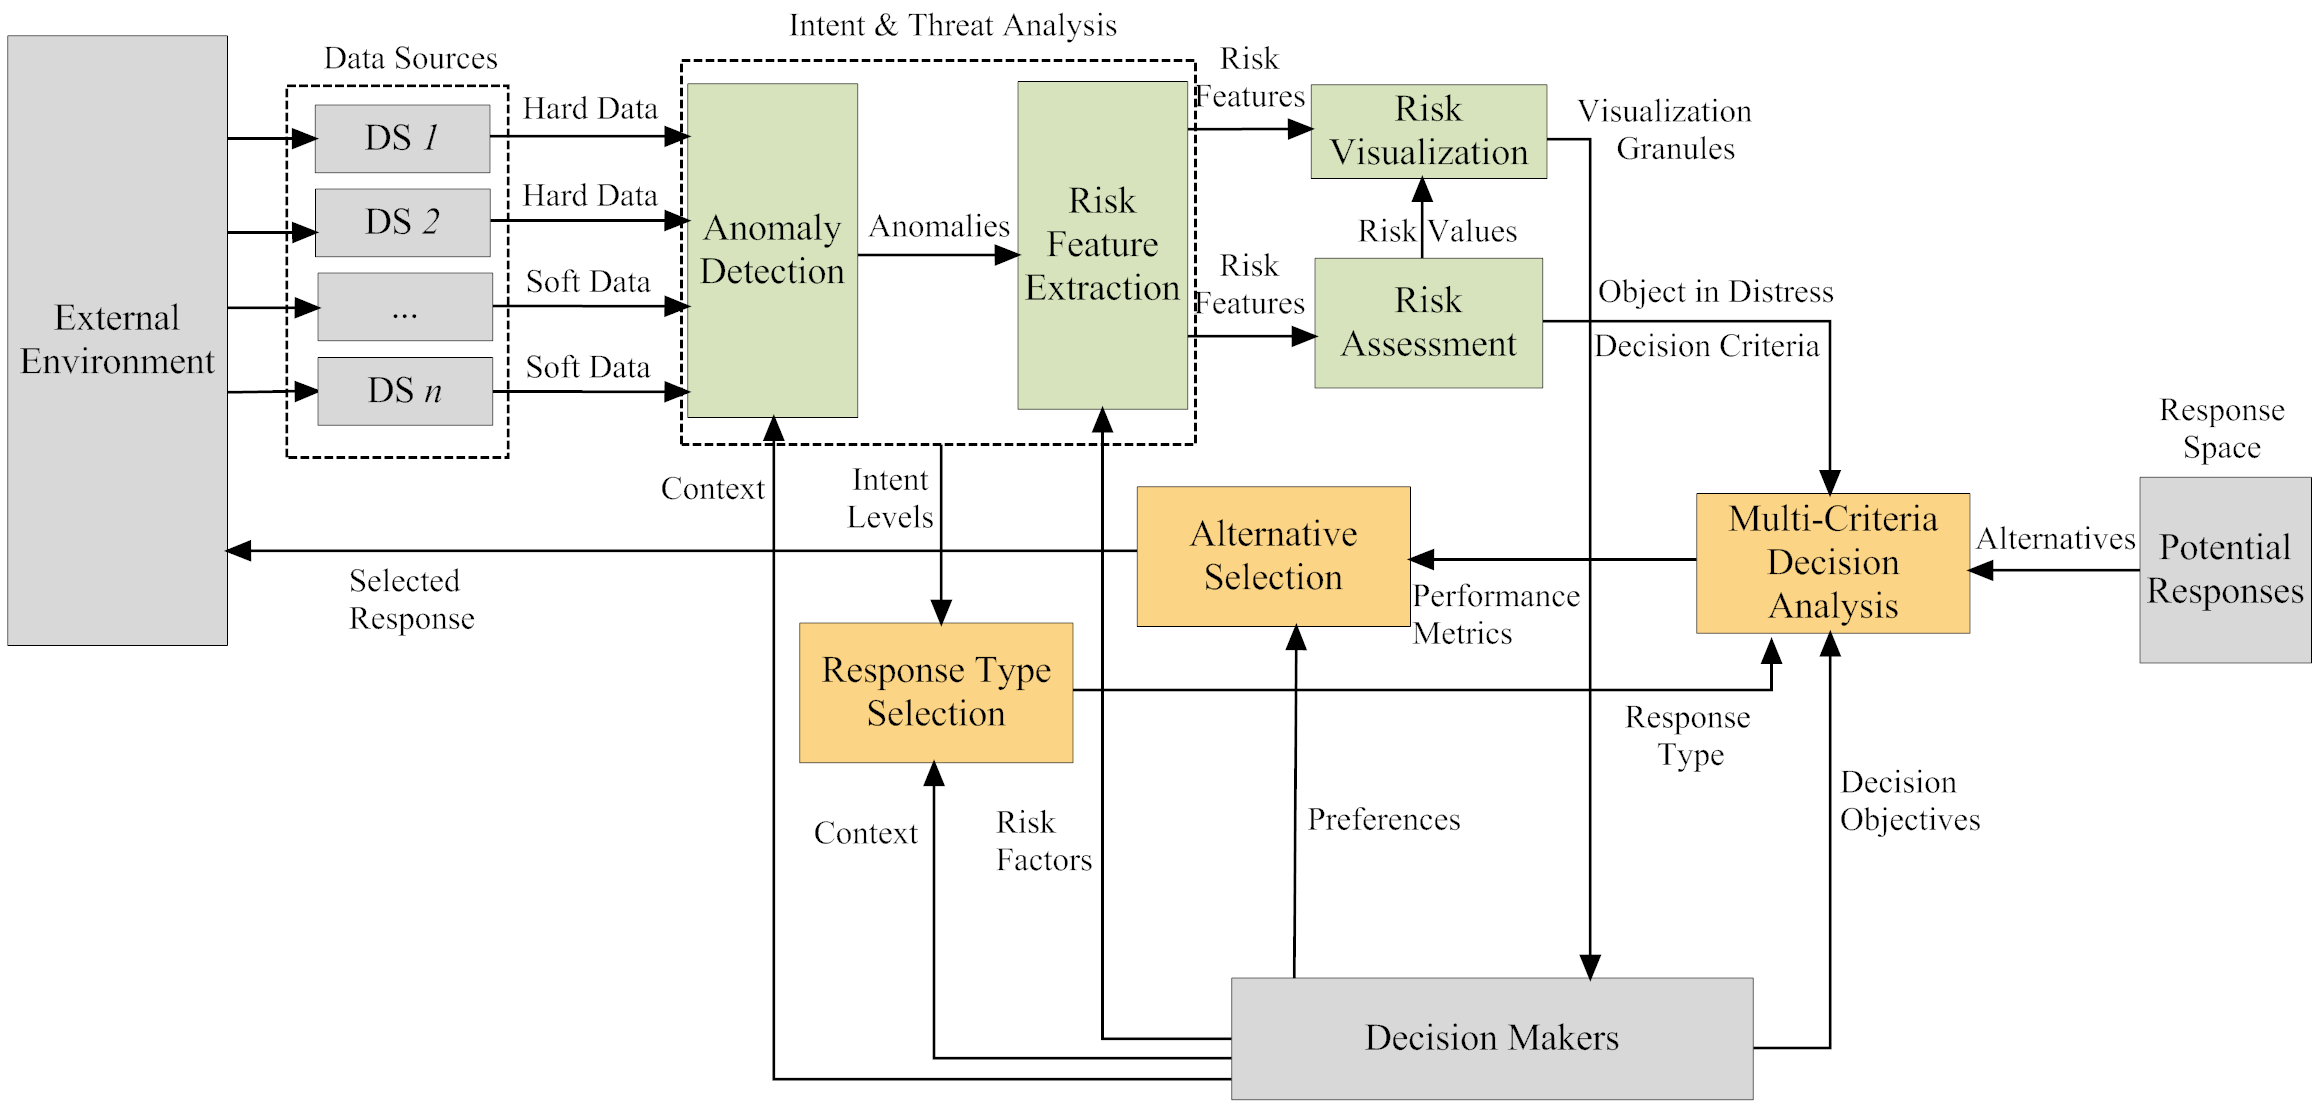
\includegraphics[width=\textwidth]{img/dataFlow-intentAnalysisRMF}}
\caption{The RMF's architectural blueprint showcasing risk feature extraction from anomalies detected in the object space. Gray boxes indicate external RMF elements. Green and yellow boxes indicate RMF's situational assessment and impact assessment capabilities, respectively.}
\label{fig:IntentAnalysisRMF}
\end{figure*}

Fig. \ref{fig:IntentAnalysisRMF} displays the proposed adaptation to the RMF in \cite{Falcon2011:RiskManagement-CIMSA} \cite{Falcon2012:ResponseAwareRMF-CEC} 

\textbf{MOO Mathematical Problem Formulation}

\section{EMOO Algorithms for RRASR}
\label{sec:Algorithms}

In this Section we unveil several common building blocks of the EMOO algorithms that will be applied to solve the RRASR problem.

\subsection{Solution Encoding}
\label{sec:Algorithms:Encoding}

\subsection{Objective Functions}
\label{sec:Algorithms:ObjFunctions}

\subsection{Evolutionary Operators}
\label{sec:Algorithms:Operators}

\subsubsection{Selection Operator}
\label{sec:Algorithms:Operators:Selection}

\subsubsection{Crossover Operator}
\label{sec:Algorithms:Operators:Crossover}

\subsubsection{Mutation Operator}
\label{sec:Algorithms:Operators:Mutation}

%\begin{algorithm}
%\caption{The custom mutation operator}
%\label{alg:Mutation}
%\begin{algorithmic}[1]
%\AlgInput a chromosome $C$, mutation probability $p_M$
%\AlgOutput the mutated chromosome $C^*$
%
%
%\For {each gene $g$ in $C$}
    %\State $r \leftarrow$ a random number $\sim U(0,1)$;
    %\If {$r < p_M$}
        %\State $g_i^* \leftarrow 1 - g_i$; \Comment{flip inclusion bit of this gene}
    %\EndIf
	  %\State $w \leftarrow$ a random number $\sim U(-1,1)$;
    %\If {$w < 0$}
        %\State corner $\leftarrow$ bottom/left side;
		%\Else
				%\State corner $\leftarrow$ top/right side;
    %\EndIf				
		%\Switch{$|w|$}
				%\Case{[0; 0.25)}
					%\State $g_r^* \leftarrow$ decrease height of $g_r$ from corner by 1;
				%\EndCase
				%\Case{[0.25; 0.5)}
					%\State $g_r^* \leftarrow$ increase height of $g_r$ from corner by 1;
				%\EndCase	
				%\Case{[0.5; 0.75)}
					%\State $g_r^* \leftarrow$ decrease width of $g_r$ from corner by 1;
				%\EndCase
				%\Case{[0.75; 1]}
					%\State $g_r^* \leftarrow$ increase width of $g_r$ from corner by 1;					
				%\EndCase
		%\EndSwitch
	%\State 	remove the added cells from the list of targets of other genes included in the solution;
	%\State add new gene $g^* = \langle g_i^*, g_r^* \rangle$ to $C^*$;
%\EndFor
%\end{algorithmic}
%\end{algorithm}

%\begin{table}[!h]
	%\centering
%\caption{Risk features extracted from both detected anomalies and available contextual information}
%\label{tab:RiskFeatures}	
  %\begin{tabular}{| l | p{2cm} | p{3cm}| } 	
    %\hline
		%\textbf{Risk Feature} & \textbf{Linguistic Term} & \textbf{Expression} \\ \hline
    %Risk$_{\text{AIS-OFF}}$ & HIGH & $\sqrt{\phi_{\text{AIS-OFF}}(X)}$ \\ \hline
		%\multirow{2}{*}{Risk$_{\text{WEATHER}}$} & LOW & $1 - \phi_{\text{BAD-WEATHER}}(X)$ \\
		%\cline{2-3} 
		%& MEDIUM & $f(\phi_{\text{BAD-WEATHER}}(X))$ \\ \hline
		%Risk$_{\text{AREA-IMPORTANCE}}$ & HIGH & $\mu(\phi_{\text{ZONES}}(X))$ Triangular [$A$=5; $B$=25; $C$=$\infty$]  \\ \hline		
		%Risk$_{\text{AREA-HOSTILITY}}$ & SIGNIFICANT & $\mu(\phi_{\text{NR-INCIDENTS}}(X)$) Trapezoidal [$A$=10; $B$=10; $C$=10; $D$=$\infty$] \\ \hline
  %\end{tabular}
%\end{table}

\subsection{Infeasibility Handling}
\label{sec:Algorithms:Infeasibility}

\subsection{Stop Criteria}
\label{sec:Algorithms:StopCriteria}



%NSGA-II will terminate after a maximum running time has elapsed. This is due to the time-critical nature of the response generation phase in our case study.

\section{Experimental Results}
\label{sec:Experiments}

This Section elaborates on the empirical evaluation of the proposed MOO methodology for the RRASR problem.

\subsection{Experimental Setup}
\label{sec:Experiments:Setup:Scenarios}

\subsubsection{Synthetic Scenario Generation}
\label{sec:Experiments:Scenarios}

\subsubsection{Algorithm and Parameter Configurations}
\label{sec:Simulations:AlgorithmsAndParameters}

\subsubsection{Performance Metrics}
\label{sec:Experiments:Metrics}

\subsection{Experiment 1: Scalability Analysis}
\label{sec:Simulations:Experiment1}

\subsection{Experiment 2: Network Density Analysis}
\label{sec:Simulations:Experiment2}

%\begin{figure}[!htbp]
%\centerline{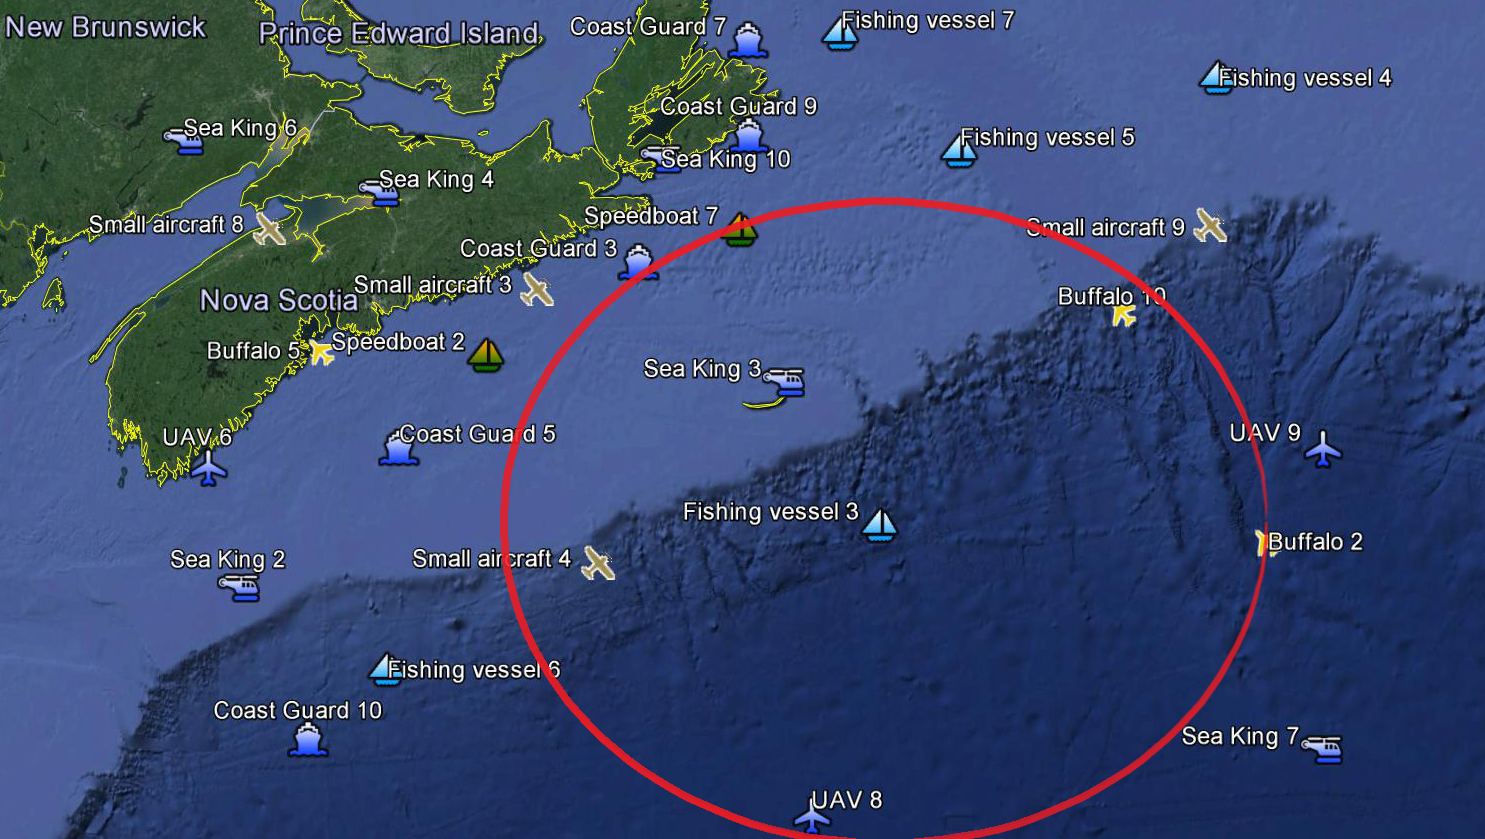
\includegraphics[width=\columnwidth]{img/scenario-vid}}
%\caption{A synthetic scenario in the Canadian Atlantic coast with 65 units: 11 small aircrafts, 10 coast guard vessels, 8 fishing vessels, 8 speedboats, 9 Sea King helicopters, 10 Buffalo search-and-rescue aircrafts and 9 unmanned aerial vehicles (UAVs). Not all units are shown in the figure. The search area is denoted by a red circle centered at the missing vessel's estimated position.}
%\label{fig:ScenarioVID}
%\end{figure}

\begin{figure}[!htbp]
\centerline{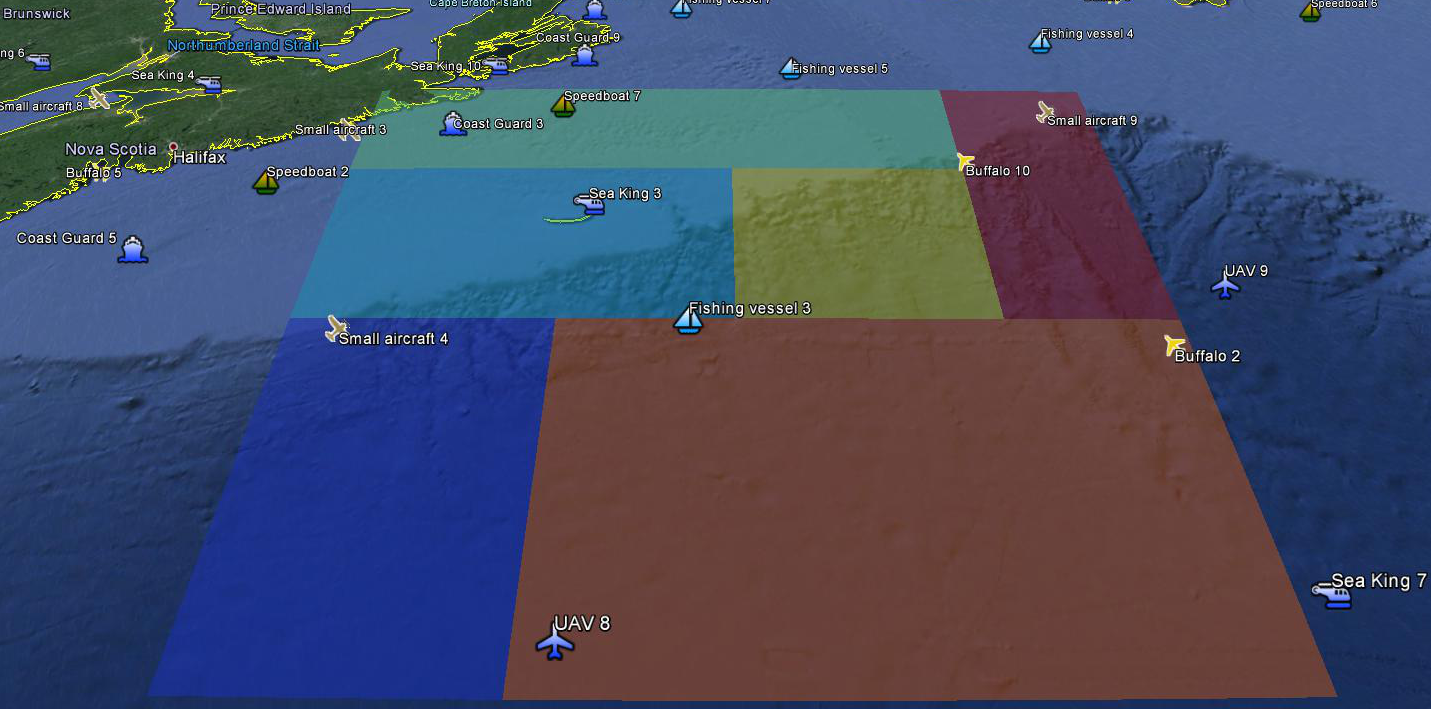
\includegraphics[width=\columnwidth]{img/response2}}
\caption{Another feasible candidate response comprising 4 maritime and 2 aerial assets. This response has high latency and low cost.}
\label{fig:Response2}
\end{figure}

\section{Conclusions}
\label{sec:Conclusions}

%We have introduced a risk-driven perspective of intent assessment and response generation, two key functionalities within High-Level Information Fusion in DSSs. The extraction of risk features from properly contextualized anomalies identified in the environment led to an interpretable characterization of the types of responses needed. The automatic generation of these responses was illustrated in the maritime realm with the case of a missing vessel.
%
%A more risk-pervasive view of the deployment environment could benefit other pivotal learning capabilities such as response assessment and process refinement. Future work will address important questions pertaining to these levels of knowledge elicitation.

\bibliographystyle{ieeetr}
\bibliography{RRASR-CEC-References}

\end{document}
